\documentclass[10pt]{beamer}

\usetheme{metropolis}
\usepackage{appendixnumberbeamer}

\usepackage{booktabs}
\usepackage[scale=2]{ccicons}

\usepackage{pgfplots}
\usepgfplotslibrary{dateplot}

\usepackage{xspace}
\newcommand{\themename}{\textbf{\textsc{metropolis}}\xspace}

\usepackage{ltablex} % Tables
\usepackage{ragged2e} % Text Alignment in Tables

\title{Empirical Research in Software Engineering}
\date{June 14, 2019}
\author{Stefan Kapferer}
\institute{University of Applied Sciences of Eastern Switzerland (HSR FHO)}

\usepackage{url}
\def\UrlNoBreaks{\do\:}

\usepackage{amsmath}

\usepackage{listings,lstautogobble}
\usepackage{minted}
\usemintedstyle{vs}

\usepackage{mathtools}

\usepackage[absolute,overlay]{textpos}
  \setlength{\TPHorizModule}{1mm}
  \setlength{\TPVertModule}{1mm}

\graphicspath{ {./images/} }

\begin{document}

\maketitle

\begin{frame}{Table of contents}
  \setbeamertemplate{section in toc}[sections numbered]
  \tableofcontents[hideallsubsections]
\end{frame}

\section{Problem \& Motivation}

\begin{frame}[standout]
	
	\textbf{Why do we need Software Engineering?}
	
\end{frame}

\begin{frame}{Software Engineering Definition}
	
	\textbf{Software engineering aims to provide systematic methods and tools to overcome the challenges we face in software development.}
	
	\begin{itemize}
		\item Software development is a complex process.
		\item It is based on human-based activities and creativity.
		\item ``Software is developed and not produced.'' \cite{10-1007-3-540-57092-6-91}
	\end{itemize}

	\bigskip
	\begin{quotation}
		``(1) The application of a systematic, disciplined, quantifiable approach to the development, operation, and maintenance of software; that is, the application of engineering to software. (2) The study of approaches as in (1).'' - IEEE \cite{159342}
	\end{quotation}
\end{frame}

\begin{frame}[standout]
	
	\textbf{Why Empirical Research in Software Engineering?}
	
\end{frame}

\begin{frame}{Why Empirical Research in Software Engineering?}
	
	\textbf{These methods and tools applied to software development evolve and change.}	
	
	\begin{itemize}
		\item Continuous improvement
		\item Evaluation of applicability and effectiveness
		\item The similarities to social and behavioral sciences do not allow to be as formal as in mathematics or physics.
		\begin{itemize}
			\item Software engineering is a discipline \textbf{highly based on human activities and creativity}.
		\end{itemize}
	\end{itemize}

\end{frame}

\begin{frame}{The Empirical Method}
	
	\textbf{Empirical research strategies can help measuring and analyzing the impact of new methods and tools in software engineering:}	

	\bigskip		
	\begin{itemize}
		\item Is a variation of the \textbf{scientific method} \cite{10-1007-3-540-57092-6-91,Glass:1994:SC:624604.625401}.
		\item Uses statistical and qualitative methods.
		\item Knowledge is gained by \textbf{observation or experiments applied to practice}.
	\end{itemize}

\end{frame}

\begin{frame}{Applying Empirical Research}
	
	\textbf{Empirical research strategies aim for understanding a phenomenon in the ``real world'' context.}	

	\begin{itemize}
		\item They can be used to evaluate results of research and thesis projects in the industry.
		\item For example: understand and analyze the capabilities of a new tool.
	\end{itemize}

\end{frame}

\section{Application Example}


\begin{frame}[fragile]{Context Mapper \cite{contextmapper}: An Example Thesis Project}
	
	\textbf{A Domain-specific Language for Context Mapping \linebreak \& Service Decomposition}\footnote{\url{https://contextmapper.github.io/}}
	
	\begin{textblock}{20}(92,12)
		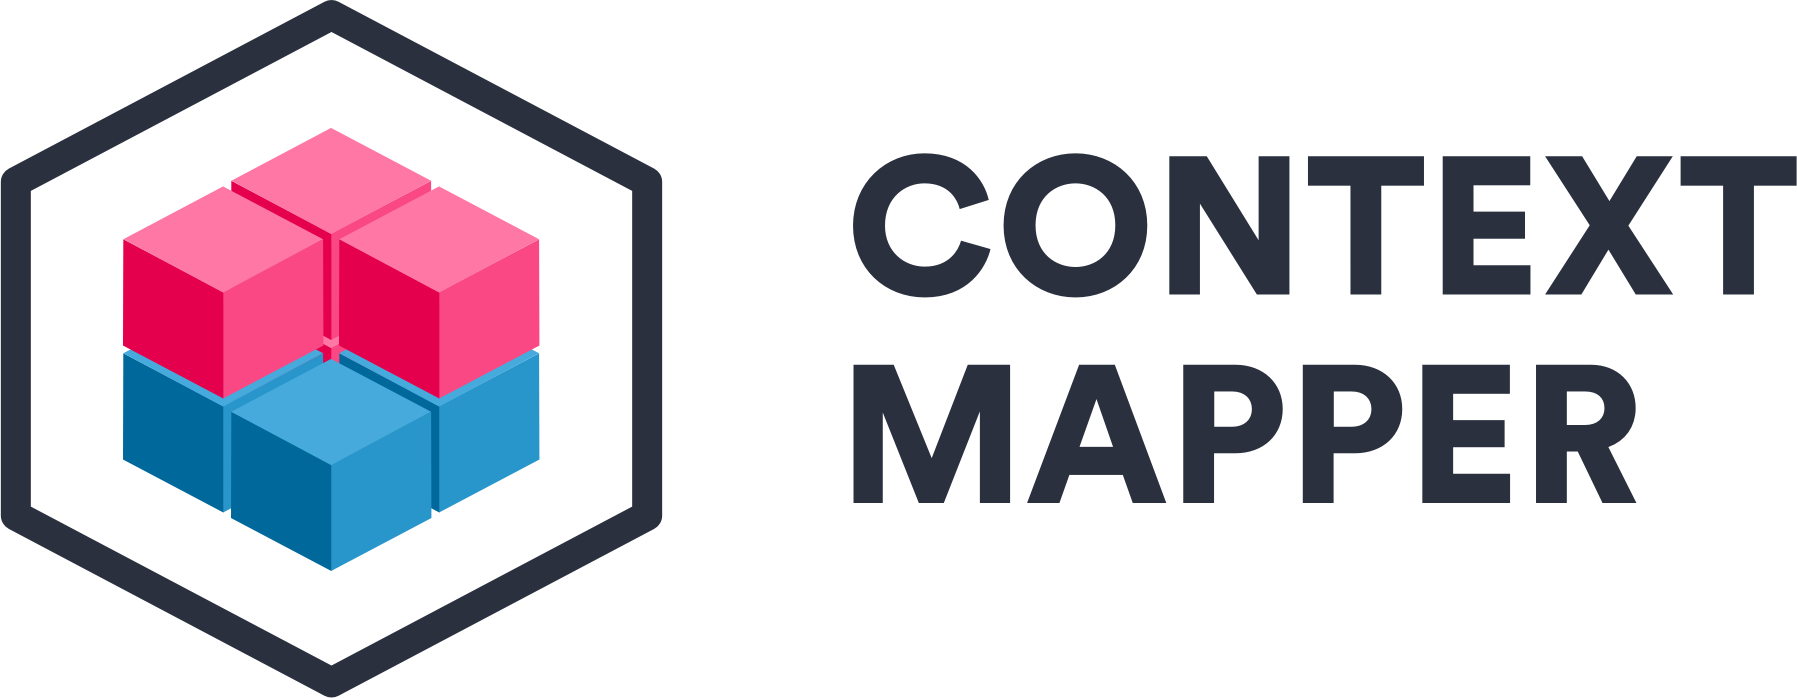
\includegraphics[scale=0.05]{./images/cm.png}
    \end{textblock}	
	
	\begin{itemize}
		\item Modeling Domain-driven Design (DDD) Context Maps
		\item Practitioners using this DDD concept have to draw these context maps by hand (no other tools available yet).
	\end{itemize}
	
\begin{minted}[frame=single,linenos,fontsize=\scriptsize]{cml-lexer.py:CMLLexer -x}
ContextMap {
  /* Add Bounded Contexts to Context Map */
  contains CustomerManagement, CustomerSelfService, DebtCollection
  
  /* Define Bounded Context Relationships: */
  
  CustomerSelfService [D,C]<-[U,S] CustomerManagement
  
  PolicyManagement [SK]<->[SK] DebtCollection
}
\end{minted}

\end{frame}

\begin{frame}{Context Mapper \cite{contextmapper}: An Example Thesis Project}
	
	\textbf{Our hypothesis}:
	\begin{quotation}
		``Software architects and DDD adopters can benefit from a tool which supports the creation of DDD-based models in a formal and expressive way. Thereby, the models can be transformed and evolved iteratively, which increases the process and productivity.''
	\end{quotation}	
	
\end{frame}

\begin{frame}{Context Mapper \cite{contextmapper}: An Example Thesis Project}
	
	\textbf{Example research questions to be answered by using empirical studies:}
	
	\bigskip
	\begin{itemize}
		\item \textbf{RQ1:} Does the tool fulfill the practitioners requirements regarding usability and expressiveness to model their context maps with the tool?
		\item \textbf{RQ2:} Does the tool reduce the effort required by the software architects and improves the productivity over the project lifecycle?
		\item \textbf{RQ3:} Which factors are relevant whether a company would use the tool or not?
	\end{itemize}
	
\end{frame}

\section{Empirical Strategies}

\begin{frame}{Overview of Empirical Strategies}
	
	\textbf{Fundamental strategies of empirical software engineering \cite{Avison:1999:AR:291469.291479,Wohlin:2012:ESE:2349018}:}
	
	\begin{figure}[H]
		\centering
		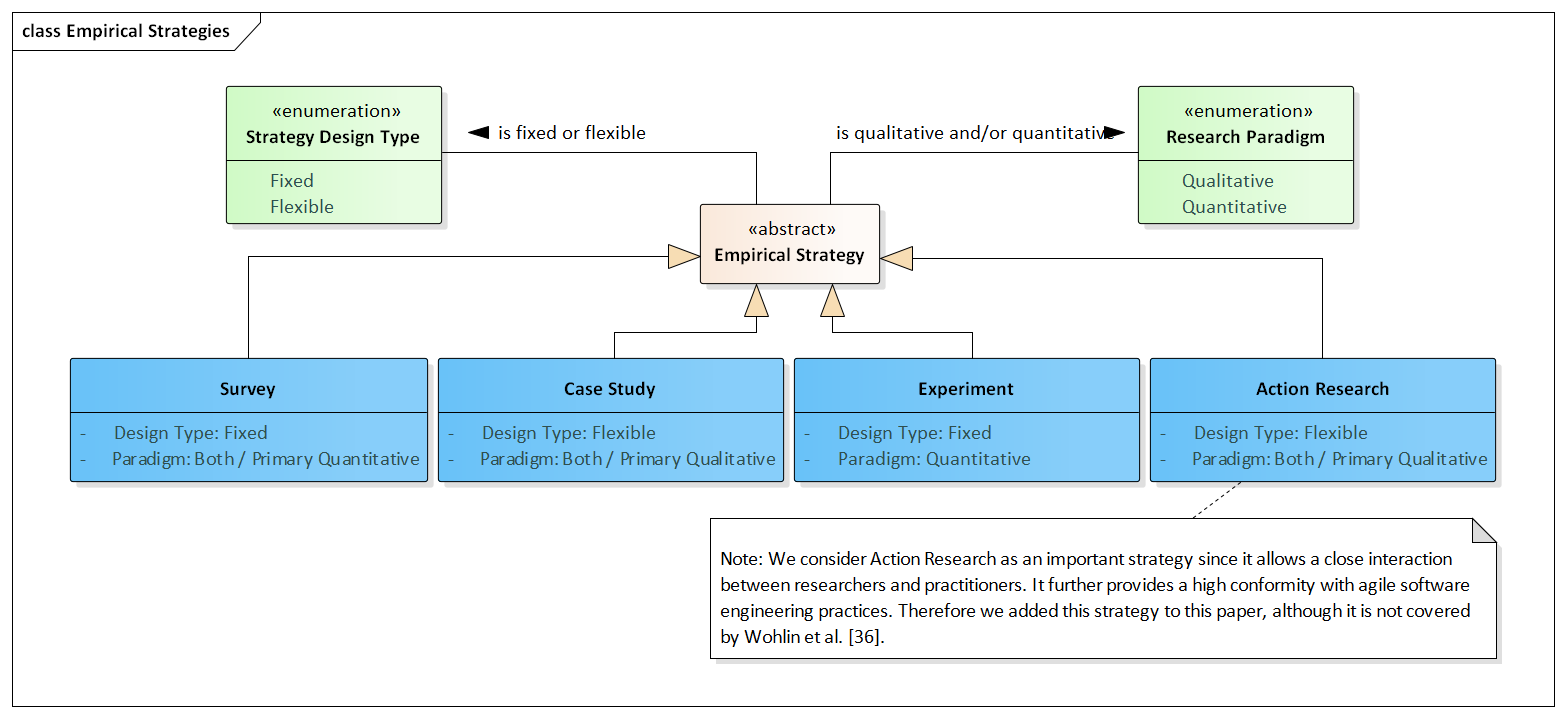
\includegraphics[width=1.0\textwidth]{Empirical_Strategies}
		\caption{Empirical Strategies in Software Engineering}
		\label{fig:empirical-strategies}
	\end{figure} 
	
\end{frame}

\begin{frame}{Survey}
	With \textbf{surveys} we can:
	
	\begin{itemize}
		\item Collect data from or about people.
		\item Derive a generalized opinion of a broad population of individuals.
	\end{itemize}	

	Surveys collect data with \textbf{questionnaires} or \textbf{interviews}.
	
	\begin{itemize}
		\item Descriptive: examine characteristics of population
		\item Explanatory: identify reasons for certain behavior
		\item Explorative: open survey where RQs are not clear yet (pre-study)
	\end{itemize}
	
\end{frame}

\begin{frame}{Survey}
	\begin{columns}[T] % align columns
		\begin{column}{.48\textwidth}
			\textbf{For example:}
			\begin{itemize}
				\item As a pre-study: What do architects think about the idea of formalizing DDD context maps? (RQ3)
				\begin{itemize}
					\item Investigate expectations of target user group.
				\end{itemize}			
				\bigskip
				\item Evaluate user impressions regarding usability and expressiveness of DSL. (RQ1)
			\end{itemize}					
		\end{column}
		\hfill
		\begin{column}{.48\textwidth}
			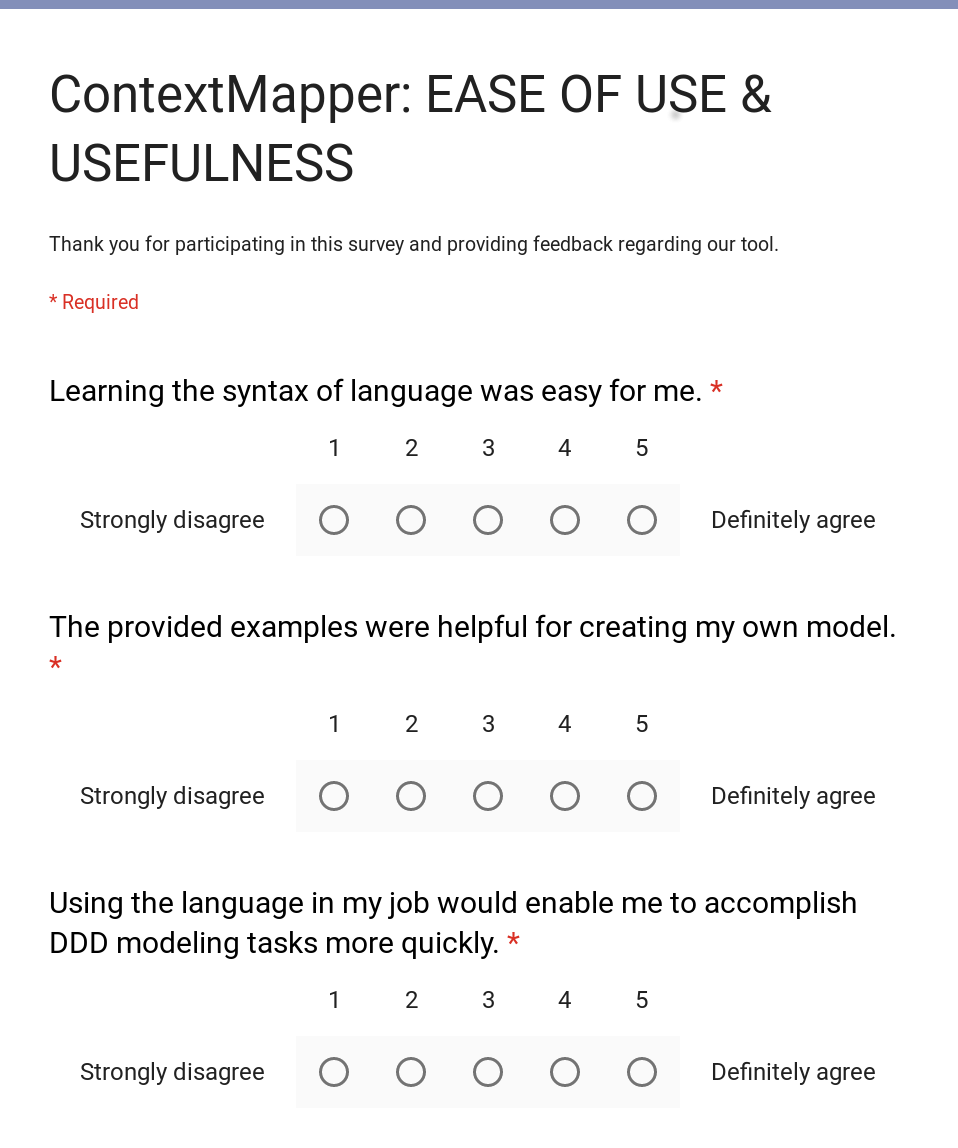
\includegraphics[width=1.0\linewidth]{./images/survey_example.png}
		\end{column}
	\end{columns}
\end{frame}

\begin{frame}{Case Study}
	
	Case studies \textbf{``investigate contemporary phenomena in their context''} \cite{Benbasat:1987:CRS:35194.35201,robson2002real,yin2009case}:
	
	\begin{itemize}
		\item Observe how a new tool or method behaves in practice.
		\begin{itemize}
			\item Apply it in an industry project.
		\end{itemize}
		\item Typically used in cases where it is not possible to isolate the phenomenon from its context.
		\item Uses the following methods to collect data:
		\begin{itemize}
			\item Interviews
			\item Observations
			\item Archival Data
		\end{itemize}
	\end{itemize}
	
\end{frame}

\begin{frame}{Case Study}

	\textbf{For example} use the Context Mapper tool in a company which already uses DDD context maps to:
	\bigskip
	\begin{itemize}
		\item Apply observation methods using A/B testing and usability tests to \textbf{detect unfulfilled requirements}. (RQ1)
		\bigskip
		\item Conduct interviews to \textbf{study user satisfaction}. (RQ1)
		\bigskip
		\item Recording user actions to \textbf{compare ``effort-completion time''}. (RQ2)
	\end{itemize}
	
\end{frame}

\begin{frame}{Action Research}
	
	Action research has \textbf{similarities to case studies}, but in this case the researcher \textbf{actively participates in the project to improve the tool or process}.
	
	\bigskip
	\begin{quotation}
		``In action research, the emphasis is more on what the practitioners do than what they say they do.'' \cite{Avison:1999:AR:291469.291479}
	\end{quotation}
	
	\begin{itemize}
		\item Experiment together with the practitioners.
		\item Use the user feedback to directly improve the tool or process.
		\item Improve and test with users again.
	\end{itemize}
\end{frame}

\section{Relationships with Agile Practices}

\begin{frame}{Relationships with Agile Practices}
	
	\textbf{What is the relationship to (agile) software engineering practices? Are combinations possible?}
	
	\bigskip
	\begin{enumerate}
		\item Software engineering approaches are the \textbf{major subject} to empirical studies in our field.
		\bigskip
		\item \textbf{Agility} of empirical strategies
		\begin{itemize}
			\item How ''agile`` are they?
			\item Is it possible to apply them and proceed in an ''agile`` manner?
		\end{itemize}
	\end{enumerate}
	
\end{frame}

\begin{frame}{How ``agile'' are these Empirical Strategies?}
	
	\textbf{Can we use the presented strategies and proceed in an ``agile'' way?}
	
	\bigskip
	Important agile practices\footnote{\url{https://www.agilealliance.org/}}:
	\begin{itemize}
		\item Ability to respond to change.
		\item Regular retrospectives.
		\item Short feedback loops with customers (practitioners).
		\item Self empowerment of development teams.
	\end{itemize}
	
\end{frame}

\begin{frame}{How ``agile'' are these Empirical Strategies?}

	\textbf{Agility of empirical strategies:}	
	
	\begin{itemize}
		\item Action research is already very agile by design.
		\item Case studies a bit less, since the researcher not participates in the project.
		\item Experiments and surveys do not conform due to their fixed design.
	\end{itemize}
	
	\textbf{Possible solution to introduce ``agility'' for all strategies:}
	\begin{itemize}
		\item Conduct smaller studies and iterate.
		\item Use results of one study as input for next one.	
	\end{itemize}		
	
	\bigskip
	\textbf{For example: (Context Mapper)}	
	\begin{itemize}
		\item Conduct multiple small case studies and proceed in an iterative way.
	\end{itemize}		
	
\end{frame}

\section{Conclusion}

\begin{frame}{Summary \& Conclusion}

	\begin{itemize}
		\item The \textbf{main concepts of empirical software engineering} are:
		\begin{itemize}
			\item Survey
			\item Case Study
			\item Experiment
			\item Action Research
		\end{itemize}
		\bigskip
		\item The approaches are \textbf{applicable to research and thesis projects} to \textbf{evaluate software engineering methods and tools}.
		\bigskip
		\item It is possible to \textbf{apply the strategies in an agile way}.
	\end{itemize}
	
\end{frame}

\begin{frame}[standout]
  Questions?
\end{frame}

\begin{frame}[standout]
  Discussion
\end{frame}

\appendix

\begin{frame}[standout]
  Appendix
\end{frame}

\begin{frame}{Experiment}
	
	Experiments provide \textbf{more control} than a case study and is typically conducted in a \textbf{laboratory environment}.
	
	\begin{itemize}
		\item In experiments researchers measure the impact of changing one or more variables.
		\item The rest of the environment must be keept at a fixed level.
		\begin{itemize}
			\item Therefore only applicable in a laboratory and not in a ``real world'' environment.
		\end{itemize}
	\end{itemize}
	
	\bigskip
	\textbf{For example:}
	\begin{itemize}
		\item Let software architects or engineers create DDD context maps in a laboratory environment.
		\item Compare \textit{time} and \textit{effort} needed to fulfill specific tasks with the tool and without the tool.
		\begin{itemize}
			\item Thereby measure if productivity increases as predicted.
		\end{itemize}
	\end{itemize}		
	
\end{frame}

\begin{frame}[allowframebreaks]{References}

  \bibliography{presentation}
  \bibliographystyle{abbrv}

\end{frame}

\end{document}
